\section{Model and experimental benchmark}\label{sec:model}

Figure~\ref{fig:model} shows the model: the actively damped milling system of \citet{ozsoy2026robust}, rebuilt from its published parameters.

\begin{figure}[!tbp]
\centering
\begin{tikzpicture}[
  >=Stealth, font=\small,
  blk/.style={draw, rounded corners=1.5pt, minimum height=9mm, align=center, fill=white},
  sum/.style={draw, circle, inner sep=1.4pt, fill=white},
  lab/.style={font=\footnotesize, inner sep=1.5pt}]
  % junctions and blocks, placed explicitly so that no wire crosses a block
  \node[sum] (s1) at (0,0) {$+$};
  \node[sum] (s2) at (0,1.7) {$+$};
  \node[blk, minimum width=21mm] (F0) at (-2.5,1.7) {static force\\ $f_s(t;a)$};
  \node[blk, minimum width=40mm] (cut) at (3.0,1.7) {regenerative force\\ $aH(t)\,[x(t)-x(t-T)]$};
  \node[blk, minimum width=17mm] (G) at (1.9,0) {structure\\ $G(s)$};
  \node[coordinate] (xb) at (5.7,0) {};
  \node[blk, minimum width=12mm] (D) at (6.9,0) {$s$};
  \node[coordinate] (vb) at (8.1,0) {};
  \node[blk, minimum width=17mm] (K) at (6.9,-1.9) {DVF\\ $-g$};
  \node[blk, minimum width=17mm] (sat) at (4.3,-1.9) {clip\\ $\sat_{\Vmax}$};
  \node[blk, minimum width=17mm] (Ga) at (1.7,-1.9) {actuator\\ $G_a(s)$};
  % cutting forces
  \draw[->] (F0.east) -- (s2.west);
  \draw[->] (cut.west) -- (s2.east);
  \draw[->] (s2.south) -- node[lab, left] {$f_c$} (s1.north);
  % structure and velocity
  \draw[->] (s1.east) -- (G.west);
  \draw (G.east) -- node[lab, above, pos=0.5] {$x$} (xb);
  \fill (xb) circle (1.2pt);
  \draw[->] (xb) -- (D.west);
  \draw[->] (xb) |- (cut.east);
  \draw (D.east) -- node[lab, above] {$\dot x$} (vb);
  % feedback loop
  \draw[->] (vb) |- (K.east);
  \draw[->] (K.west) -- node[lab, above] {$u$} (sat.east);
  \draw[->] (sat.west) -- node[lab, above] {$V$} (Ga.east);
  \draw[->] (Ga.west) -| node[lab, left, pos=0.75] {$f_a$} (s1.south);
  \node[lab, below=1mm of sat, text=black!60] {$|V|\le\SI{9}{\volt}$};
\end{tikzpicture}
\caption{The controlled cut. The workpiece mode $G(s)$ is driven by the cutting force $f_c$ and by the force $f_a$ of the proof-mass actuator [Eqs.~\eqref{eq:eom} and \eqref{eq:split}]. The direct velocity feedback command $u=-g\dot x$ is clipped at $\Vmax=F_{\max}/K_a=\SI{9}{\volt}$.}
\label{fig:model}
\end{figure}


\subsection{Structure, actuator and clipped velocity feedback}\label{sec:model-loop}

The workpiece is flexible in one direction, normal to the feed, and is represented by its dominant mode, with modal mass $m$, damping $c=2\zeta m\omega_n$ and stiffness $k$ (Table~\ref{tab:case}). With $x(t)$ the displacement at the cutting point and $q(t)$ the internal coordinate of the proof-mass actuator,
\begin{equation}\label{eq:eom}
  m\ddot x+c\dot x+kx=f_c(t)+f_a(t),\qquad
  \ddot q+2\zeta_a\omega_a\dot q+\omega_a^2q=V(t),\qquad
  f_a=K_a\ddot q ,
\end{equation}
where $f_c$ is the cutting force on the workpiece and $f_a$ the actuator force, so that $G(s)=1/(ms^2+cs+k)$ and $G_a(s)=K_as^2/(s^2+2\zeta_a\omega_as+\omega_a^2)$. The controller is DVF through this inertial actuator \citep{elliott2001feedback}, $u(t)=-g\dot x(t)$, and the applied command is clipped:
\begin{equation}\label{eq:dvf}
  V(t)=\operatorname{sat}_{V_{\max}}\bigl(u(t)\bigr)=\max\bigl\{-V_{\max},\,\min\{V_{\max},u(t)\}\bigr\},
\end{equation}
with $V_{\max}=F_{\max}/K_a=\SI{9}{\volt}$. While the clip is inactive the loop is linear, with the closed-loop receptance
\begin{equation}\label{eq:Gcl}
  G_{\mathrm{cl}}(s)=\frac{G(s)}{1+g\,s\,G_a(s)\,G(s)} .
\end{equation}
The clip is the only actuator limit in the model: the rated force $F_{\max}$ enters only through $\Vmax$ and is not a strict force limit, and neither stroke nor current limits are modelled (Supplementary Material, Section~\ref{S-supp:std-model-act}).
% src: src/params.py, src/structure.py; README §4.6 (clip before the actuator)

\subsection{Regenerative force of the helical cutter}\label{sec:model-force}

The cutter, with $N_t=4$ teeth, radius $R=D/2$ and helix angle $\eta$, turns at $\Omega=2\pi n/60$ and cuts to the axial depth $a$. The immersion angle of tooth $j$ at height $z\in[0,a]$ above the tool tip is
\begin{equation}\label{eq:phi}
  \phi_j(t,z)=\Omega t+2\pi j/N_t-z\tan\eta/R ,\qquad j=0,\dots,N_t-1.
\end{equation}
In half-immersion down milling a tooth cuts, $\gamma_j(t,z)=1$, while $\phi_j\in[\pi/2,\pi]$ (modulo $2\pi$), and $\gamma_j=0$ otherwise. The chip thickness of the slice $\mathrm dz$ is
\begin{equation}\label{eq:chip}
  h_j(t,z)=f_z\sin\phi_j-\bigl[x(t)-x(t-T)\bigr]\cos\phi_j ,
\end{equation}
with $T$ the tooth period, and the feed-normal force on the workpiece is
\begin{equation}\label{eq:fcut}
  f_c(t)=-\sum_{j=0}^{N_t-1}\int_0^a\gamma_j\,\bigl(K_{tc}\sin\phi_j-K_{rc}\cos\phi_j\bigr)\max\{h_j,0\}\,\mathrm dz ,
\end{equation}
so the force vanishes where the tool loses contact. As long as every engaged chip is positive, $f_c$ splits into a static and a regenerative part,
\begin{align}
  f_c(t)&=f_s(t;a)+aH(t)\,\bigl[x(t)-x(t-T)\bigr],\label{eq:split}\\
  aH(t)&=\sum_{j=0}^{N_t-1}\int_0^a\gamma_j\,\bigl(K_{tc}\sin\phi_j\cos\phi_j-K_{rc}\cos^2\phi_j\bigr)\,\mathrm dz ,\label{eq:aHt}
\end{align}
where $f_s$ is Eq.~\eqref{eq:fcut} with $h_j=f_z\sin\phi_j$; both are $T$-periodic, and the mean coefficient is exactly linear in the depth \citep{altintas1995analytical}:
\begin{equation}\label{eq:aHmean}
  \begin{aligned}
    \overline{aH}&=\frac{N_tK_{tc}\,a}{4\pi}\,\alpha_{yy},\\
    \alpha_{yy}&=2\int_{\pi/2}^{\pi}\Bigl(\sin\phi\cos\phi-\frac{K_{rc}}{K_{tc}}\cos^2\phi\Bigr)\mathrm d\phi
    =-1-\frac{\pi}{2}\,\frac{K_{rc}}{K_{tc}}=-1.428 ,
  \end{aligned}
\end{equation}
with $\alpha_{yy}$ the directional factor.
% src: src/zoa.py (alpha_matrix), src/tdsim.c (force), src/c3_periodic.py (aH); verification/zoa_sdm/README.md §1 (derivation, alpha_yy = -1.428399)

\subsection{Linear stability limit}\label{sec:model-zoa}

Replacing $aH(t)$ by its mean, the zero-order approximation (ZOA) of \citet{altintas1995analytical}, and linearising the deviation from the forced orbit of Section~\ref{sec:model-orbit} gives the characteristic equation
\begin{equation}\label{eq:char}
  1-\frac{N_tK_{tc}\,a}{4\pi}\,\alpha_{yy}\bigl(1-e^{-i\omega T}\bigr)\,G_{\mathrm{cl}}(i\omega)=0 .
\end{equation}
At a fixed speed, $a_{\lim}(g)$ is the smallest real positive depth $a(\omega)$ given by Eq.~\eqref{eq:char}; it is conservative by at most about \SI{1}{\percent} with respect to the time-periodic helical model (Supplementary Material, Section~\ref{S-app:simulator}).
% src: src/zoa.py (F_GRID; pole guard); README §2-3; verification/zoa_sdm/current_grid_check.json (table_96: 1.96e-5); README §3 and Appendix A (time-periodic model: ZOA conservative by 0-1.04 %)

\subsection{Forced orbit and its command}\label{sec:model-orbit}

Below $\alim$ and with the command inside the clip, the motion converges to a $T$-periodic forced orbit $x_p(t)$. On this orbit the regenerative term of Eq.~\eqref{eq:split} vanishes, so $x_p$ is the response of the linear loop \eqref{eq:Gcl} to the static force alone. As every slice carries the static force per unit depth of the slice at $z=0$, $\hat f_s(\theta)=\sum_m\hat f_m\,e^{imN_t\theta}$ with $\theta=\Omega t$ the spindle angle, delayed by its helix lag $z\tan\eta/R$, the integral over the depth is exact:
\begin{equation}\label{eq:Fm}
  F_m(a)=\hat f_m\,\frac{1-e^{-imN_ta\tan\eta/R}}{imN_t\tan\eta/R}\quad(m\neq0),\qquad F_0(a)=\hat f_0\,a .
\end{equation}
With $\omega_T=2\pi/T=N_t\Omega$, the orbit and its command are
\begin{equation}\label{eq:xp}
  x_p(t)=\sum_{m=-N_h}^{N_h}G_{\mathrm{cl}}(im\omega_T)\,F_m(a)\,e^{im\omega_Tt},\qquad
  b(t)=-g\,\dot x_p(t).
\end{equation}
The orbit persists unchanged in the clipped loop as long as its peak command $\bmax=\max_t\lvert b(t)\rvert$ stays below $\Vmax$, and $\Vmax-\bmax$ is then the authority left for any deviation from the orbit.
% src: src/feasibility.py (slice_force_harmonics, force_harmonics, forced_velocity)

\subsection{Case study and experimental benchmark}\label{sec:model-case}

The flexible direction, not stated in the text of \citet{ozsoy2026robust}, is taken normal to the feed, which reproduces their uncontrolled stability chart (median deviation \SI{0.04}{\percent} over \SIrange{400}{3000}{\rpm}), and the damping ratio is \SI{1.34}{\percent} rather than the \SI{1.45}{\percent} of their Table~1, because the receptance, pole and stability chart computed in that paper are fitted by the former.
% src: README §2, §4.1, §5.1, §6; verification/consistency/a_damping.json (fig6a peak -111.10 dB, model -111.10 dB at 1.34 % and -111.79 dB at 1.45 %; fig6b pole 1.3405 %; fig9 fit 1.3394 %); results/paper_vs_ours.json (p05: 0.037 % at 1.34 %)

At the gains used in their tests, the linear limit classifies 17 of the 19 distinct published cuts as measured. The two exceptions, controlled cuts that chattered below the predicted limit at \SI{1300}{\rpm} and \SI{10}{\milli\metre} ($0.80\alim$) and at \SI{2800}{\rpm} and \SI{5.5}{\milli\metre} ($0.76\alim$), do not chatter in the clipped model either: step and face entries settle at both, and the critical kick is 25--\SI{27}{\milli\metre\per\second} over 16 kick phases at \SI{1300}{\rpm}, whereas no kick up to \SI{3}{\metre\per\second} causes chatter at \SI{2800}{\rpm}. Saturation-induced finite-amplitude instability (Section~\ref{sec:bistability}) thus cannot explain the second cut, and explains the first only if the test contained a perturbation of that size, which neither simulated entry produces. The tool is rigid, the mode uniform over the depth and the loop, outside Section~\ref{sec:delayed}, without delay; the depths and kicks reported below are predictions of this model (Supplementary Material, Section~\ref{S-supp:std-model-case}).
% src: results/cuts_main.json (21 marks, 19 distinct cuts; pred_paper equals measured at 17/19; 1300 rpm, 10 mm: g_paper 1157.98 V s/m, alim_paper 12.478 mm (10/12.478 = 0.80); 2800 rpm, 5.5 mm: g_paper 679.55 V s/m, alim_paper 7.264 mm (5.5/7.264 = 0.76))
% src: verification/paper/revision_runs.json (published_cuts_entries: step and face entries, 9 V clip, full surface memory (NREG = 0), chatter false at both cuts; published_cuts_kicks_mps: 1300 rpm 0.02505-0.02673 m/s over 16 phases, 2800 rpm inf at all 16 phases, i.e. no kick of DV_GRID up to DV_HI = 3 m/s (src/c1_unsafe_zone.py))

\begin{table}[!tbp]
  \centering
  \caption{Case-study parameters \citep{ozsoy2026robust}. Quantities marked $^\dagger$ are derived from the others; those marked $^\ddagger$ are chosen or inferred in this work (Section~\ref{sec:model-case}); Table~1 of \citet{ozsoy2026robust} lists $\zeta=\SI{1.45}{\percent}$. Symbols: Supplementary Material, Table~\ref{S-tab:nomenclature}.}
  \label{tab:case}
  \small
  \begin{tabular}{@{}lll@{}}
    \toprule
    Quantity & Symbol & Value\\
    \midrule
    \multicolumn{3}{@{}l}{\emph{Structure: one mode, feed-normal direction}}\\
    Natural frequency & $\omega_n/2\pi$ & \SI{129.3}{\hertz}\\
    Modal stiffness & $k$ & \SI{1.34e7}{\newton\per\metre}\\
    Modal mass$^\dagger$ & $m=k/\omega_n^2$ & \SI{20.30}{\kilogram}\\
    Damping ratio$^\ddagger$ & $\zeta$ & \SI{1.34}{\percent}\\
    \multicolumn{3}{@{}l}{\emph{Proof-mass actuator and command}}\\
    Force constant & $K_a$ & \SI{3}{\newton\per\volt}\\
    Actuator coefficients & $2\zeta_a\omega_a$; $\omega_a^2$ & \SI{15.834}{\per\second}; \SI{2785.6}{\per\second\squared}\\
    Actuator mode$^\dagger$ & $\omega_a/2\pi$; $\zeta_a$ & \SI{8.40}{\hertz}; 0.150\\
    Peak force & $F_{\max}$ & \SI{27}{\newton}\\
    Command limit$^\dagger$ & $V_{\max}=F_{\max}/K_a$ & \SI{9}{\volt}\\
    \multicolumn{3}{@{}l}{\emph{Cutter and cutting conditions}}\\
    Diameter; teeth; helix & $D$; $N_t$; $\eta$ & \SI{16}{\milli\metre}; 4; \SI{45}{\degree}\\
    Axial tooth pitch$^\dagger$ & $p_a$ & \SI{12.57}{\milli\metre}\\
    Cutting coefficients & $K_{tc}$; $K_{rc}$ & \SI{660}{\mega\pascal}; \SI{180}{\mega\pascal}\\
    Radial immersion & $a_e/D$ & 0.5, down milling\\
    Feed per tooth & $f_z$ & \SI{0.05}{\milli\metre}\\
    Directional factor$^{\dagger\ddagger}$ & $\alpha_{yy}$ & $-1.428$\\
    Spindle speeds & $n$ & \SIrange{500}{3000}{\rpm}, step \SI{10}{\rpm}\\
    \multicolumn{3}{@{}l}{\emph{Numerical settings}}\\
    Simulation & & 512 steps/rev, 30 layers\\
    Harmonics of the orbit$^\ddagger$ & $N_h$ & 40\\
    Gain search interval$^\ddagger$ & $\mathcal G$ & $[0,1500]$ or $[0,3000]$ \si{\volt\second\per\metre}\\
    \bottomrule
  \end{tabular}
\end{table}
% src: src/params.py (Table 1, Table 2, Eq. 3, RPM_GRID, STEPS_PER_REV, N_REVS, N_LAYERS, FLEX_DIR); src/feasibility.py (N_HARM); src/gainmap.py (G = [0, 3000]); README §2

\subsection{A second data set on the same rig}\label{sec:model-second}

For the same set-up, \citet{ozsoy2025frequency} give 39 controlled cuts with DVF at $g=\SI{253}{\volt\second\per\metre}$ on the structure of Table~\ref{tab:case}, reported stable, marginal or chattering, and 56 tests at 1700--\SI{2200}{\rpm} after re-clamping the workpiece, with the measured amplitude of the command or the mark that the actuator saturated (Supplementary Material, Sections~\ref{S-supp:std-model-second} and~\ref{S-supp:oz25}). They form a second data set on the same rig, not a second machine.
% src: verification/ozsoy2025/setup2025.py (Table 2 of the 2025 article = src/params.py; RECLAMPED 128.1 Hz, 1.48 %, 1.13e7 N/m), digitise_notes.md, points_fig6.json, points_fig10.json

The linear model reproduces their uncontrolled and controlled stability charts to 0.04 and \SI{0.14}{\milli\metre} (RMS, outside the steep flanks of the lobes) for the first structure and to 0.06 and \SI{0.07}{\milli\metre} for the second. Of the 39 controlled cuts, the model and their chart classify the same 26 as measured.
% src: verification/ozsoy2025/setup2025.py (Table 2 of the 2025 article = src/params.py), digitise_notes.md, points_fig6.json, points_fig10.json; verification/ozsoy2025/fit_gain.py/.json (fig6: uncontrolled rms 0.040 mm, controlled_g253 rms 0.137 mm; fig10_uncontrolled rms 0.062 mm; fig10_gain_fit g_best 251, rms_at_253 0.074 mm); compare2025.py/.json and a recomputation with the digitised controlled curve of Fig. 6 (26 of 39 classified as measured by both)

For the 36 unsaturated tests, the settled forced demand $K_ag\max\lvert\dot x_p\rvert$ is 0.90 times the measured amplitude (median; interquartile range 0.83--1.02), and within \SI{2.5}{\newton} of it at the 16 tests of up to \SI{5}{\milli\metre} at 1700--\SI{2000}{\rpm} (Fig.~\ref{fig:oz25}b). At \SI{15}{\milli\metre} it is about twice the measured value, and at 2050--\SI{2200}{\rpm} the measured command at 2--\SI{3}{\milli\metre} is 1.1 to 2.3 times the prediction. The settled cut is predicted to saturate at 4 of the 20 saturated tests; the command reaches the clip during the simulated face entry at 12 of them, and later at two more, through simulated chatter above the controlled limit.
% src: verification/ozsoy2025/forced_map.py (demand_components), sim2025.py/.json, compare2025.py/.json (fig10.amplitude_peak: n 36, median_ratio_pred_over_meas 0.903, ratio_q25_q75 0.832-1.021; abs_error_depth_le5_rpm_le2000_N: n 16, max 2.46; demand_over_measured.depth_15: median 2.05 (1.23-2.64); measured over predicted at 2050-2200 rpm, 2-3 mm: 1.09-2.34 (recomputed from rows); saturation_settled_closed_form both 4 of 20; saturation_any_time_face_entry both 14, pred_only 2); clip during the face entry at 12 of the 14 run_clipped Sat tests, at 2050/10 and 2100/10 only after full engagement (sim2025_fig10.json entry_peak_demand_N 17.3 and 13.5 N, run peak 337 and 353 N)

Relative to the model's linear limits (Fig.~\ref{fig:oz25}a), all 37 tests below the uncontrolled limit settled, 10 of them saturated. Between the two limits, 5 of the 7 saturated tests chattered or were marginal, and none of the 6 unsaturated ones did (one-sided Fisher exact test, $p=0.016$; for chatter alone, 2 of 7 against 0 of 6, $p=0.27$); above the controlled limit the 3 saturated tests chattered, while 3 unsaturated ones at 1700--\SI{1800}{\rpm} and 20--\SI{22}{\milli\metre}, above the model's and the published controlled limit, were stable. The model does not reproduce the 5 losses of stability between the limits: it predicts their settled command at 12--\SI{19}{\newton}, except at \SI{1950}{\rpm} and \SI{20}{\milli\metre} (\SI{33}{\newton}), both simulated entries settle, and, with kicks at four phases, a kick of at most \SI{3}{\metre\per\second} ends in chatter at only two of them, both marginal, with impulses $m\Delta v^*$ (re-clamped modal mass, \SI{17.4}{\kilogram}) of 1.7 and 2.3 times the cutting impulse of one tooth period [Eq.~\eqref{eq:impulse}]. \citet{ozsoy2025frequency} report disagreement with their own frequency-domain model at 2050--\SI{2200}{\rpm}, which they relate to loss of contact of the actuator or other nonlinearities; for the first structure, their time-domain simulation, whose details are not given, places the onset of saturation at \SI{2100}{\rpm} at \SI{4.5}{\milli\metre}, where the forced demand of the present model is \SI{13.5}{\newton}. The saturation tests are thus consistent with the mechanism of this paper: below the controlled limit, losses of stability occurred only above the uncontrolled limit and only in tests whose command saturated. As a cut that chatters also drives the command into the clip, and the article does not say when during a test the command saturated, the data cannot show that the saturation came first.
% src: verification/ozsoy2025/compare2025.json (fig10.by_position: below a_lim(0) n 37, sat 10, unstable 0; between n 13; above a_lim(g) n 6, chatter 3, sat 3; between_sat_vs_outcome 5/2 against 0/6, fisher_one_sided_p 0.0163; rows: 1700/20, 1750/20, 1800/22 stable above a_lim(g)); kicks2025.py/.json (13 points between the limits: finite at 2000/10 (138.7 mm/s, marginal) and 1950/20 (396.5 mm/s, marginal), inf at the other 11); onset2025.py/.json (first structure, squares of the article's Fig. 6; 2100 rpm: article onset 4.5 mm, demand there 13.5 N, no model onset below a_lim(g) = 7.78 mm); article Sec. 4.2 (disparity at 2050-2200 rpm, 'actuator loss of contact effects or other nonlinearities'); kicks at phases 0, 4, 8, 12 of 16 (kicks2025.py PHASES; crit_by_phase_mmps finite at all four phases at 1950/20 and 2000/10, none at 2050/5, 2100/5, 2150/5); impulse ratio m dv*/(Fbar_y T) with the re-clamped m = 17.44 kg and Eq. (16): 2.419/1.452 = 1.67 at 2000 rpm / 10 mm, 6.916/2.979 = 2.32 at 1950 rpm / 20 mm; Fisher one-sided for chatter alone 462/1716 = 0.269

\begin{figure}[!tbp]
  \centering
  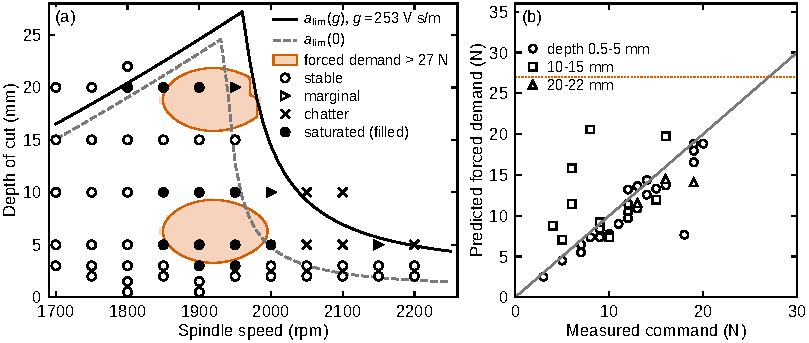
\includegraphics[width=\textwidth]{figures/fig_oz25.pdf}
  \caption{Saturation tests of \citet{ozsoy2025frequency} (their Figs.~10 and 12; re-clamped structure, DVF, gain not stated) against the model with $g=\SI{253}{\volt\second\per\metre}$. (a)~Linear limits of the model, uncontrolled (dashed) and controlled (solid); shaded: settled forced demand above \SI{27}{\newton} (the \SI{9}{\volt} clip) below the controlled limit; markers: measured outcome, filled where the command saturated (every chattering test saturated). (b)~Predicted settled forced demand against the measured command amplitude at the 36 unsaturated tests, by depth; solid: equality; dotted: \SI{27}{\newton}.}
  \label{fig:oz25}
\end{figure}
% src: paper/figures/make_figures.py fig_oz25 (verification/ozsoy2025/forced_map_reclamped_g253.npz, compare2025.json)
